\documentclass[a4paper]{jpconf}
\usepackage{graphicx}
\begin{document}
\title{An efficient, modular and simple tape archiving solution for LHC Run-3}

\author{S Murray\textsuperscript{1}, V Bahyl\textsuperscript{1}, G Cancio\textsuperscript{1}, E Cano\textsuperscript{1}, V Kotlyar\textsuperscript{2}, D F Kruse\textsuperscript{1}, and J Leduc\textsuperscript{1}}

\address{\textsuperscript{1}European Organization for Nuclear Research CERN, CH-1211 Gen\`eve 23}
\address{\textsuperscript{2}Institute for High Energy Physics, Russian Federation State Research Centre (IHEP), RU-142 281 Protvino Moscow Region, Russia}

\ead{\{Steven.Murray, Vladimir.Bahyl, German.Cancio.Melia, Eric.Cano, Daniele.Francesco.Kruse, Julien.Leduc\}@cern.ch and Victor.Kotlyar@ihep.ru}

\begin{abstract}
The IT Storage group at CERN develops the software responsible for archiving to
tape the custodial copy of the physics data generated by the LHC experiments.
Physics run 3 will start in 2021 and will introduce two major challenges for
which the tape archive software must be evolved. Firstly the software will need
to make more efficient use of tape drives in order to sustain the predicted data
rate of 150 petabytes per year as opposed to the current 50 petabytes per year.
Secondly the software will need to be seamlessly integrated with EOS, which has
become the de facto disk storage system provided by the IT Storage group for
physics data.

The tape storage software for LHC physics run 3 is code named CTA (the CERN Tape
Archive). This paper describes how CTA will introduce a pre-emptive drive
scheduler to use tape drives more efficiently, will encapsulate all tape
software into a single module that will sit behind one or more EOS systems, and
will be simpler by dropping support for obsolete backwards compatibility.
\end{abstract}

\section{Introduction} \label{introduction}

The IT Storage group (IT-ST) at CERN is currently designing and developing the
CERN Tape Archive (CTA) storage system.  CTA is the natural evolution of the
CERN Advanced STORage manager (CASTOR\cite{CASTOR}) with which the IT-ST
group have had many years of operational and development experience
\cite{experiences}.  The primary goal of CTA is to provide the EOS\cite{EOS} disk
storage system with a tape backend.  EOS is the de facto disk storage system for
physics data at CERN.  EOS combined with CTA will eventually replace CASTOR
which is the current system used to archive physics data to tape.  The IT-ST
group plans to put CTA into production by the beginning of 2019, ready for
experiments to start migrating to it during the long shut down period between
LHC physics runs 2 and 3.

In 2016, LHC physics run 2 archived over 50 petabytes of physics data to tape
using CASTOR.  The data rates of LHC physics run 2 will increase up to 100
petabytes per year during 2017 and 2018.

LHC physics run 3 will start in 2021 and is predicted to store over 150
petabytes per year.  Run 3 will use EOS and CTA as opposed to CASTOR to archive
data to tape.  The CTA project will increase tape drive utilization in order to
deal with the predicted 150 petabytes of physics data per year.  CTA
will accomplish this by introducing a pre-emptive scheduler that will keep
tape drives running at full speed \cite{new} all of the time.  Physics data on
tape are not only accessed by physicists.  These data are read back for data
verification and read and re-written for tape media repack\cite{repack}
campaigns. A repack campaign reads data from older lower capacity tapes and
writes them to newer higher capacity tapes.  This enables the CERN computing
centre to store more data whilst occupying the same amount of floor space. The
pre-emptive scheduler will improve tape drive efficiency by automatically
filling otherwise idle tape drive time with background jobs for data
verification and tape media repacking.

The next two sections are intended to give a more concrete idea of what is CTA.
Section \ref{cta_architecture} describes the architecture of CTA and lists the
steps taken to archive a file to tape and then to retrieve it back to disk.
Section \ref{concepts} describes the concepts that an operator needs to
understand in order to configure and work with CTA.  Section \ref{scheduler}
describes the pre-emptive drive scheduler of CTA and how it will enable the IT
storage group of CERN to handle the 150 petabytes per year transfer rate of LHC
physics run 3.  Section \ref{migrating} describes how and when LHC experiments
and other users of CASTOR will migrate to EOS and CTA.  Finally, section
\ref{conclusion} draws the paper to a close with its conclusions.

\section{CTA architecture} \label{cta_architecture}

Figure \ref{architecture} shows many EOS instances communicating with a single
CTA instance.  Each LHC experiment at CERN has its own EOS disk storage system
and its own set of tapes.  The tape drives are shared by all of the experiments
in order to be cost effective.  During any one day, an individual tape drive
may mount and transfer data to and from tapes belonging to many different
experiments.

\begin{figure}[h]
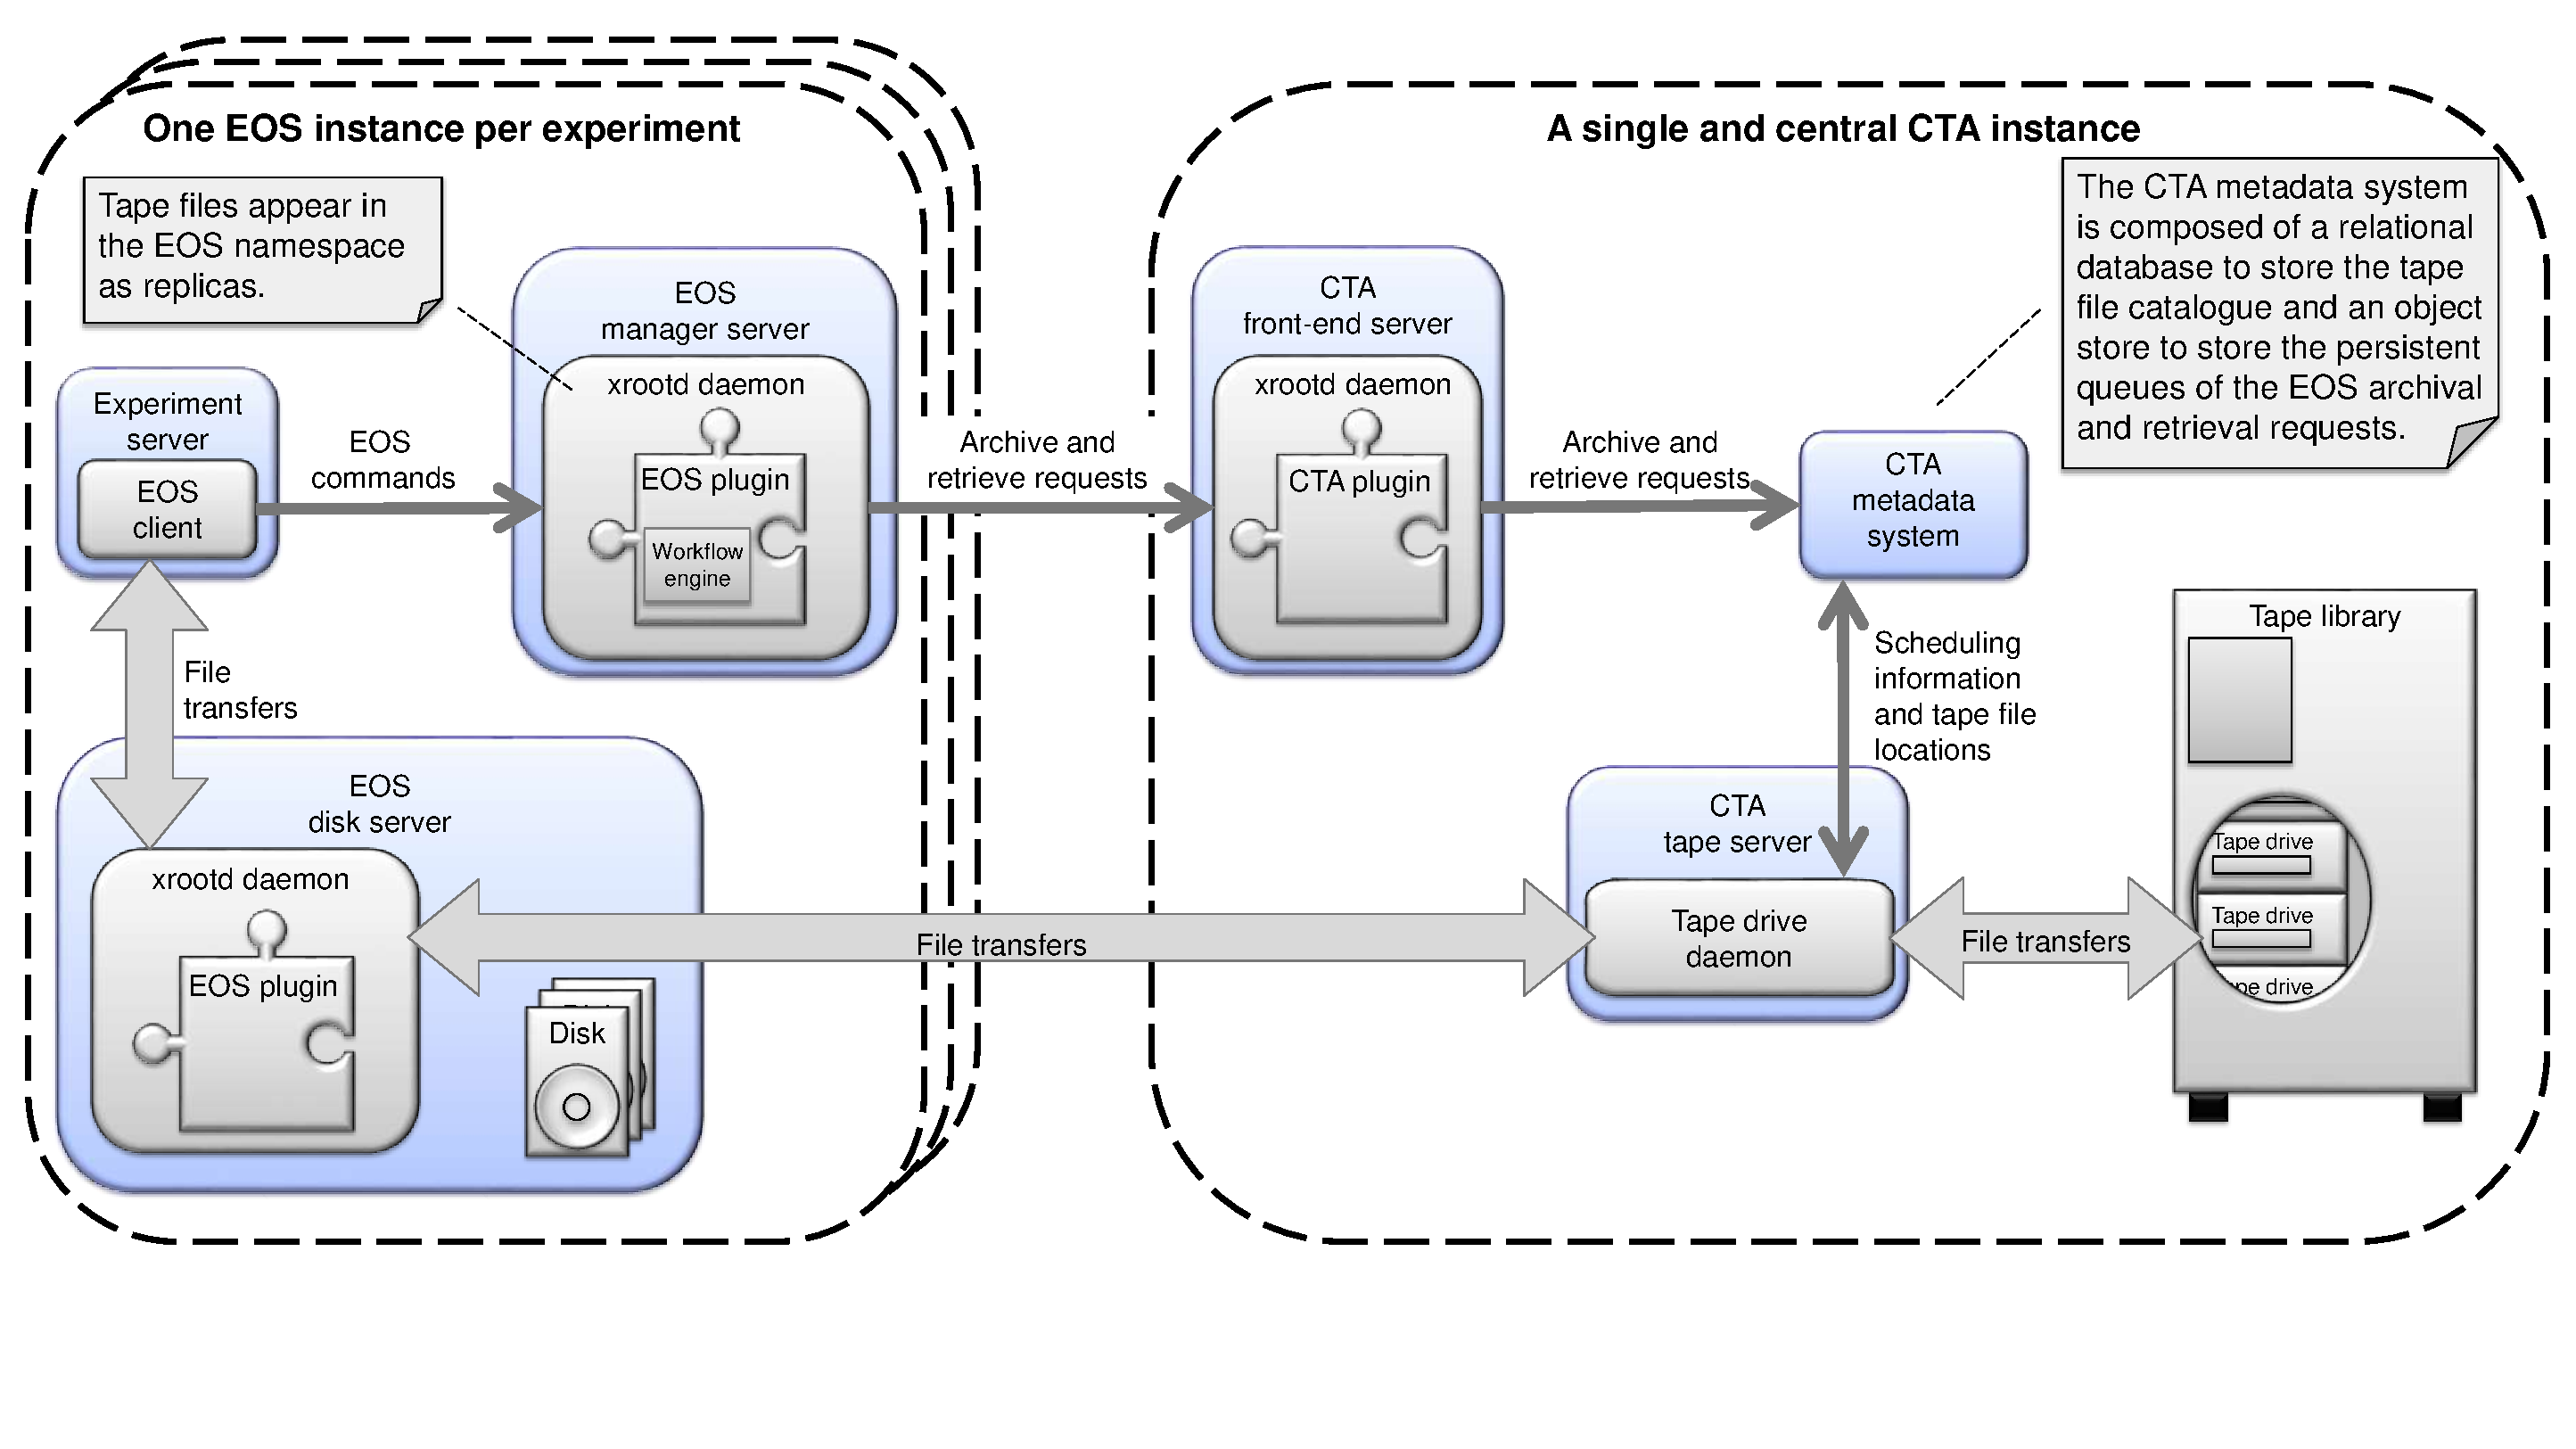
\includegraphics[width=\textwidth, trim=0mm 35mm 0mm 0mm, clip]{CTA_architecture_A4.pdf}
\caption{\label{architecture}The EOS and CTA architecture}
\end{figure}

Starting on the left hand side of figure \ref{architecture}.  EOS clients such
as the \texttt{eos} and \texttt{xrdcp} command-line tools send commands to the
EOS manager server and transfer the contents of files to and from EOS disk
servers.  EOS users see their files on tape as additional replicas.  For example
the \texttt{eos file info} command will display the tape replica of a given EOS
file.

In addition to its normal EOS duties, the EOS manager server also queues
requests with the CTA front-end in order to have EOS disk files archived to tape
or retrieved back to disk.  The EOS workflow engine is the internal EOS
component that is responsible for queuing requests with the CTA front-end.  The
EOS workflow engine and its configuration form the glue that holds EOS and CTA
together.

The EOS workflow engine can be configured to provide end users with the
following different storage system behaviours.
\begin{itemize}
  \item D1T0 - Disk only files.
  \item D1T1 - Files replicated on both disk and tape.
  \item D0T1 - Tape files cached on disk.
  \item Explicit tape file retrievals.
  \item Implicit tape file retrievals.
\end{itemize}
In the case of an explicit tape file transfer, a user issues a bring on-line
request for an EOS file that is on tape but not on EOS disk.  They poll EOS
until the file has been retrieved from tape.  Once the file has been retrieved,
the user accesses the file on EOS disk.  In the case of an implicit tape
retrieval, a user is blocked when they try to open an EOS file that is on tape
but not on EOS disk.  They are unblocked when the file has been retrieved from
tape.

Moving to the middle of figure \ref{architecture}.  The CTA front-end server
provides a network based interface to EOS and the CTA administration tool used
by tape operators (not shown).  The CTA front-end stores requests from EOS in
the persistent CTA metadata system.  The CTA front-end also queries the CTA
metadata system in order to answer the query commands of the CTA administration
tool.

The CTA metadata system is composed of two parts.  A relational database to
store the tape file catalogue and an object store to persistently queue data
transfer requests from EOS.  A relational database was chosen for the tape file
catalogue in order to minimise risk.  Relational database technology has a
proven track record of being able to safely store and recover in the event of a
disaster, mission critical information such as the location of every LHC physics
file on tape.  An object store was chosen to implement the persistent queues of
CTA because without special tricks, relational database tables do not perform
well when their rows are continuously inserted and deleted as is the case for a
queue.

The CTA tape drive daemon was copied and evolved from CASTOR.  CTA benefits from
the experience of CASTOR including how to control tape hardware and how to queue
transfer requests in order to use tape hardware efficiently.  The CTA tape drive
daemon queries the CTA metadata system for tapes to be mounted and files to be
transferred.  The daemon transfers files between tapes and the EOS disk servers.
When the daemon has completed a transfer, it writes the result back to the CTA
metadata system.

The next two subsections explain step by step how a file is archived to tape and
how a file is retrieved back to EOS disk.

\pagebreak
\subsection{Archiving a file to tape}

The following steps describe how a file is archived to tape:
\begin{enumerate}
  \item The user writes the file to EOS disk.
  \item On the close of the file, the EOS workflow engine queues a request to
  archive the file with the CTA front-end.
  \item The CTA front-end stores the archive request in the CTA metadata system.
  \item The file becomes eligible for archival.  Either the file has been
  queued for the maximum permissible amount of time or there is enough data to
  be transferred to warrant the cost of mounting a tape.
  \item A tape server connected to a free tape drive queries the CTA metadata
  system for more work and determines a tape needs to be mounted for writing.
  \item The tape server sends a request to the tape library to mount the tape.
  \item Whilst the tape is still being mounted the tape server queries the CTA
  metadata system for the files to be written to the tape.
  \item Still whilst the tape is being mounted, the tape server starts to read
  the file from EOS disk into main memory.
  \item The tape is mounted into the tape drive.
  \item The tape server starts to write the file from main memory to tape.
  \item On the close of the tape file the tape server stores the destination
  tape and file position into the CTA metadata system and notifies EOS that the
  file is safely archived.
  \item EOS updates its file namespace to reflect the fact that the file is now
  safely archived.
\end{enumerate}

\subsection{Retrieving a file from tape}

The following steps describe how a file is retrieved from tape.
\begin{enumerate}
  \item The user sends EOS a prepare request that instructs EOS to retrieve a
  file from tape.
  \item The EOS workflow engine queues the corresponding retrieve request with
  the CTA front-end.
  \item The CTA front-end stores the retrieve request in the CTA metadata
  system.
  \item The file becomes eligible for recall.  Either the file has been
  queued for the maximum permissible amount of time or there is enough data to
  be transferred to warrant the cost of mounting a tape.
  \item A tape server connected to a free tape drive queries the CTA metadata
  system for more work and determines a tape needs to be mounted for reading.
  \item The tape server sends a request to the tape library to mount the tape.
  \item The tape is mounted into the tape drive.
  \item The tape server queries the CTA metadata system for the files to be read
  from the tape.
  \item The tape server starts transferring the file from tape to EOS disk.
  \item On the close of the disk file, EOS updates its namespace to reflect the
  fact that there is now a replica of the file back on EOS disk.
\end{enumerate}

\section{Configuration and operations concepts} \label{concepts}
This section is divided into two subsections whose combined goal is to further
explain CTA by describing the concepts an operator needs to understand in order
to accomplish two typical operator tasks.  The first subsection describes the
concepts required to specify which EOS disk file gets archived to which set of
tapes.  The second subsection covers the concepts required to give users a
tailored quality of service.

\subsection{The concepts behind routing EOS disk files to tape}
An operator needs to understand the following three concepts in order to be able
to route EOS disk files to specific tape pools:
\begin{itemize}
  \item CTA storage class.
  \item Tape pool.
  \item Archive route.
\end{itemize}
An EOS user archives a file to tape by copying the file into an EOS directory
that has been tagged with a CTA storage class.  Within the EOS namespace a CTA
storage class is simply a name.  For example the \texttt{raw\_data} storage
class could be used to refer to user files that should have one copy on tape and
should be written to tapes that are dedicated to raw physics data.  Within CTA a
storage class name is mapped to the number of required copies on tape and to as
many archive routes.  An archive route specifies to which tape pool a copy of
a file should be written to. A tape pool is a logical grouping of tapes.  For
example the \texttt{raw\_data\_of\_experiment\_A} tape pool could contain all of
the tapes owned by experiment A that are dedicated to storing raw physics data.
A storage class specifying two copies on tape will have two associated archive
routes, one for each copy to be written to tape.  This enables operators to
create two destination tape pools, each one in a different physical location.

\subsection{The concepts behind giving users a tailored quality of service} 
An operator needs to understand the following two concepts in order to tailor
the quality of service delivered to EOS users and groups:
\begin{itemize}
  \item Mount policy.
  \item Mount rule.
\end{itemize}
Mounting and dismounting a tape to read or write a single file costs a
considerable amount of tape drive time and should be minimised.  Mounting a
tape, positioning it for reading or writing, rewinding it and dismounting it can
take 4 minutes.  The tape drives used at CERN have data transfer rates of around
300 megabytes per second.  4 minutes is therefore equivalent to transferring 72
gigabytes worth of data.

CTA transfers files to and from tape asynchronously so that it can queue up
enough file transfers to warrant the cost of mounting, positioning, rewinding
and dismounting a tape.  Files are copied to and read from tape in batches.

An operator creates named mount policies in order to define the following:
\begin{itemize}
  \item Mount priority: which mounts have higher priority than which.
  \item Maximum amount of time a file transfer can be kept pending.
  \item Drive quota: The maximum number tape drives that can be used when the
  system is under load.
\end{itemize}

An operator creates mount rules in order to assign mount policies to EOS users
and groups. 

\section{The pre-emptive tape drive scheduler} \label{scheduler}
CTA does not utilize a central daemon for scheduling. Instead the scheduler is a
shared software component, running as needed on the front ends and in the tape
servers. The scheduler routines store and retrieve data from the two persistent
stores of CTA: the tape file catalogue for keeping track of tapes, tape pools,
archive routes, mount policies and tape files, and the object store for keeping
track of the queued archive and retrieve jobs, as well as tape drives statuses.

\subsection{Request queuing}
When an EOS instance requests a new file transfer, the tape file catalogue is
queried to get routing information for an archival or tape file locations for a
retrieval. A transfer job is then added to the corresponding queue in the object
store. For archiving, jobs are queued per tape pool, while for retrieves, they
are attached to one tape at a time. Each queue also keeps track of the summary
of the jobs it contains to allow efficient mount scheduling.

\subsection{Tape mount scheduling and job handling}
Several competing requirements need to be taken into account when scheduling tape
drives.  User-initiated accesses in both directions should be executed within a
bound latency (measured in the order of hours). Mounting and dismounting a tape
cartridge to and from a drive can take several minutes.  The execution of a data
access is therefore postponed until the amount of data to transfer makes it
worthwhile or the job age is too high. User initiated mounts create an irregular
demand, driven by the accelerator cycles and experiment data taking, as well as
various analysis patterns.

The maintenance tasks of retrieving and archiving for repack, and retrieving for
data verification are high bandwidth tasks with very relaxed latency
requirements which could extend to several months. These low priority tasks
should get drive time when user-initiated tasks are not using the drives.

When a drive is idle and ready, the tape daemon process retrieves the summaries
of all the non-empty queues from the object store and picks the highest priority
queue that can be served by the drive. The mounts already in progress in other
drives are  also taken into account, in order to implement the drive quotas of
mount policies. This scheduling is done  atomically: at any point in time, only
one drive takes a scheduling decision.

Once a mount is started, the tape daemon just consumes the jobs from the queue and
executes them.

This single step scheduling allows flexibility with the scheduling rules and
adjustments are expected as experience with CTA grows.

\subsection{Tape drive pre-emption}
A background task that repacks or verifies a whole tape can take several hours.
Such long duration background tasks must be pre-empted when higher priority user
tasks arrive in order to meet the latency requirements of users.  A pre-empted
background task will be resumed at a later point in time when it again becomes
the highest priority task.  The tape daemon will keep polling the scheduling
information at a low rate and interrupt a low priority background task if a
higher priority one is available to replace it.

This mixing of high and low priority tasks previously had to be handled by hand or \textit{ad hoc}
scripts in CASTOR.

\subsection{CTA to EOS communication and other operations}
The scheduler is responsible for reporting the steps in the life cycle of each
file.  It coordinates the updating of the file catalogue, and EOS.

Finally, the scheduler component handles queue listing and other house keeping
tasks initiated through the front end by operators, via a command line tool.

\pagebreak
\section{Migrating from CASTOR to EOS and CTA} \label{migrating}

Figure \ref{current} gives a very high level view of how experiments transfer
files to and from tape today using CASTOR.  CASTOR and EOS are used by the
experiments as separate Grid storage elements.  Experiments use EOS to store
the files they actively work on and modify.  Experiments use CASTOR to archive
files to tape.  Files can also be transferred directly between EOS and CASTOR
without having to go via an experiment.

\begin{figure}[h]
\centering
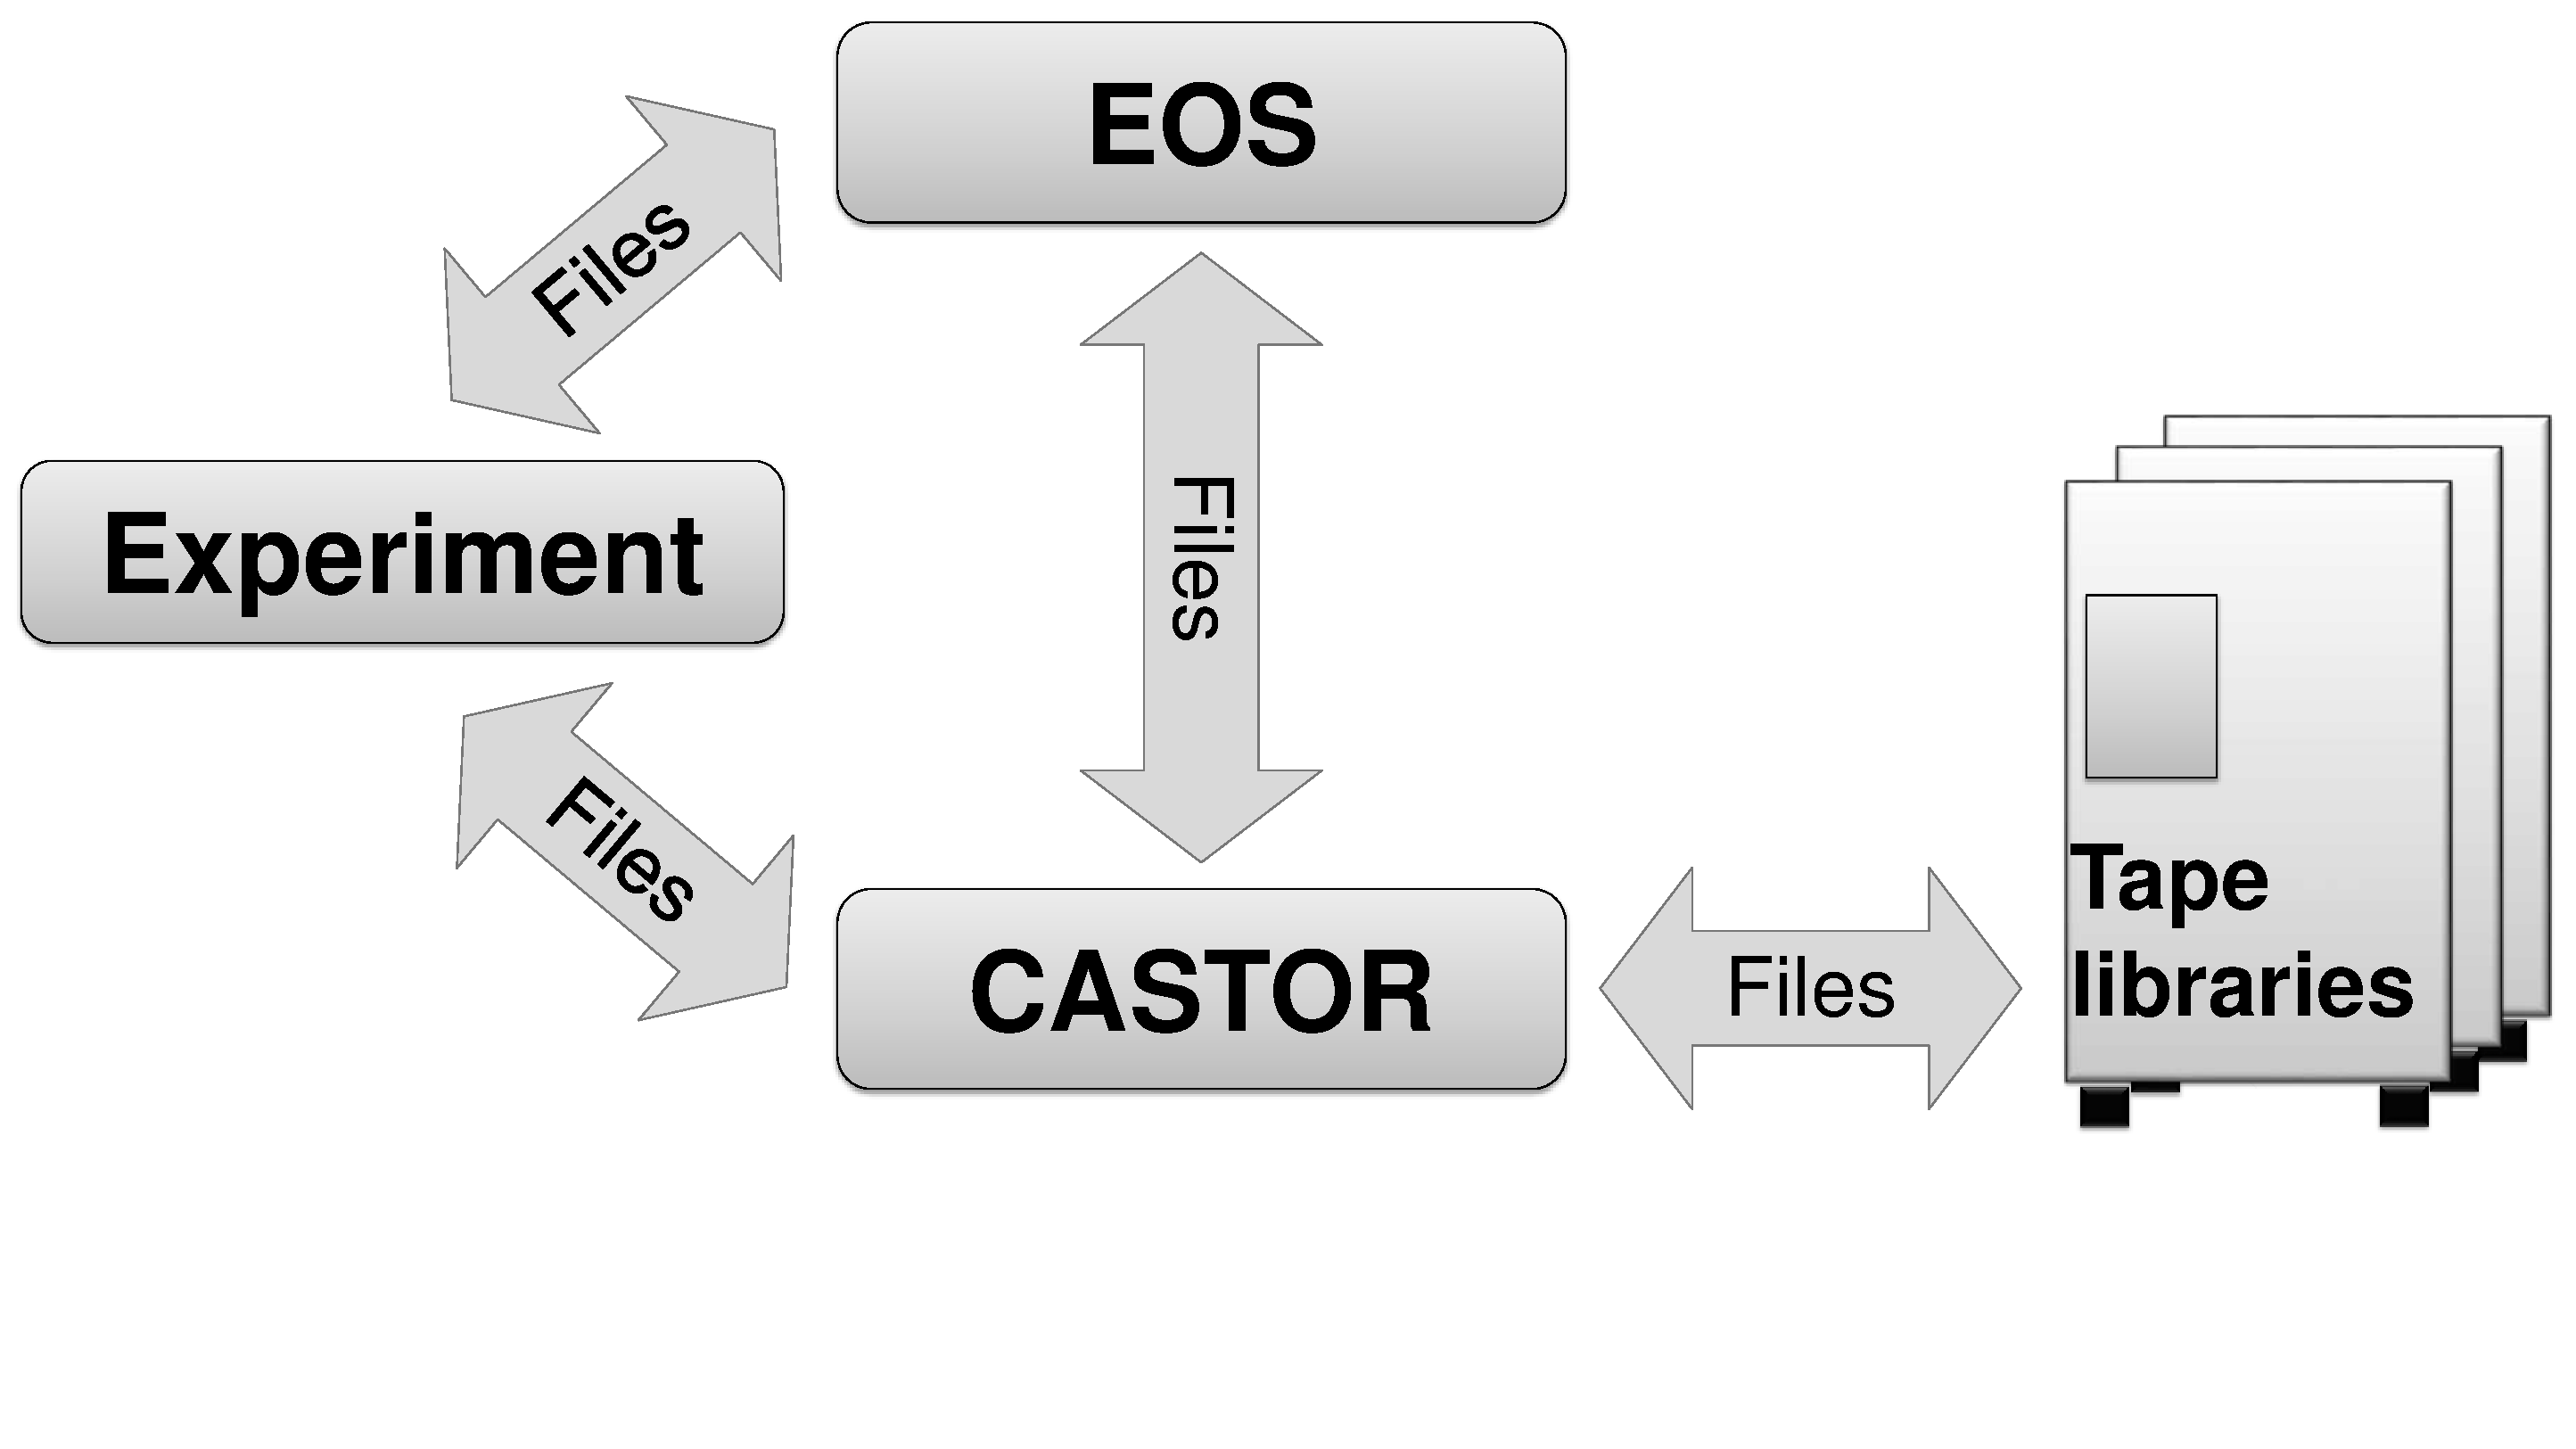
\includegraphics[scale=0.18, trim=0mm 60mm 0mm 0mm, clip]{CTA_current_deployment.pdf}
\caption{\label{current}The current deployment of CASTOR}
\end{figure}

Figure \ref{replacement} shows that an EOS instance together with CTA will be
a drop in replacement for a CASTOR storage element.

\begin{figure}[h]
\centering
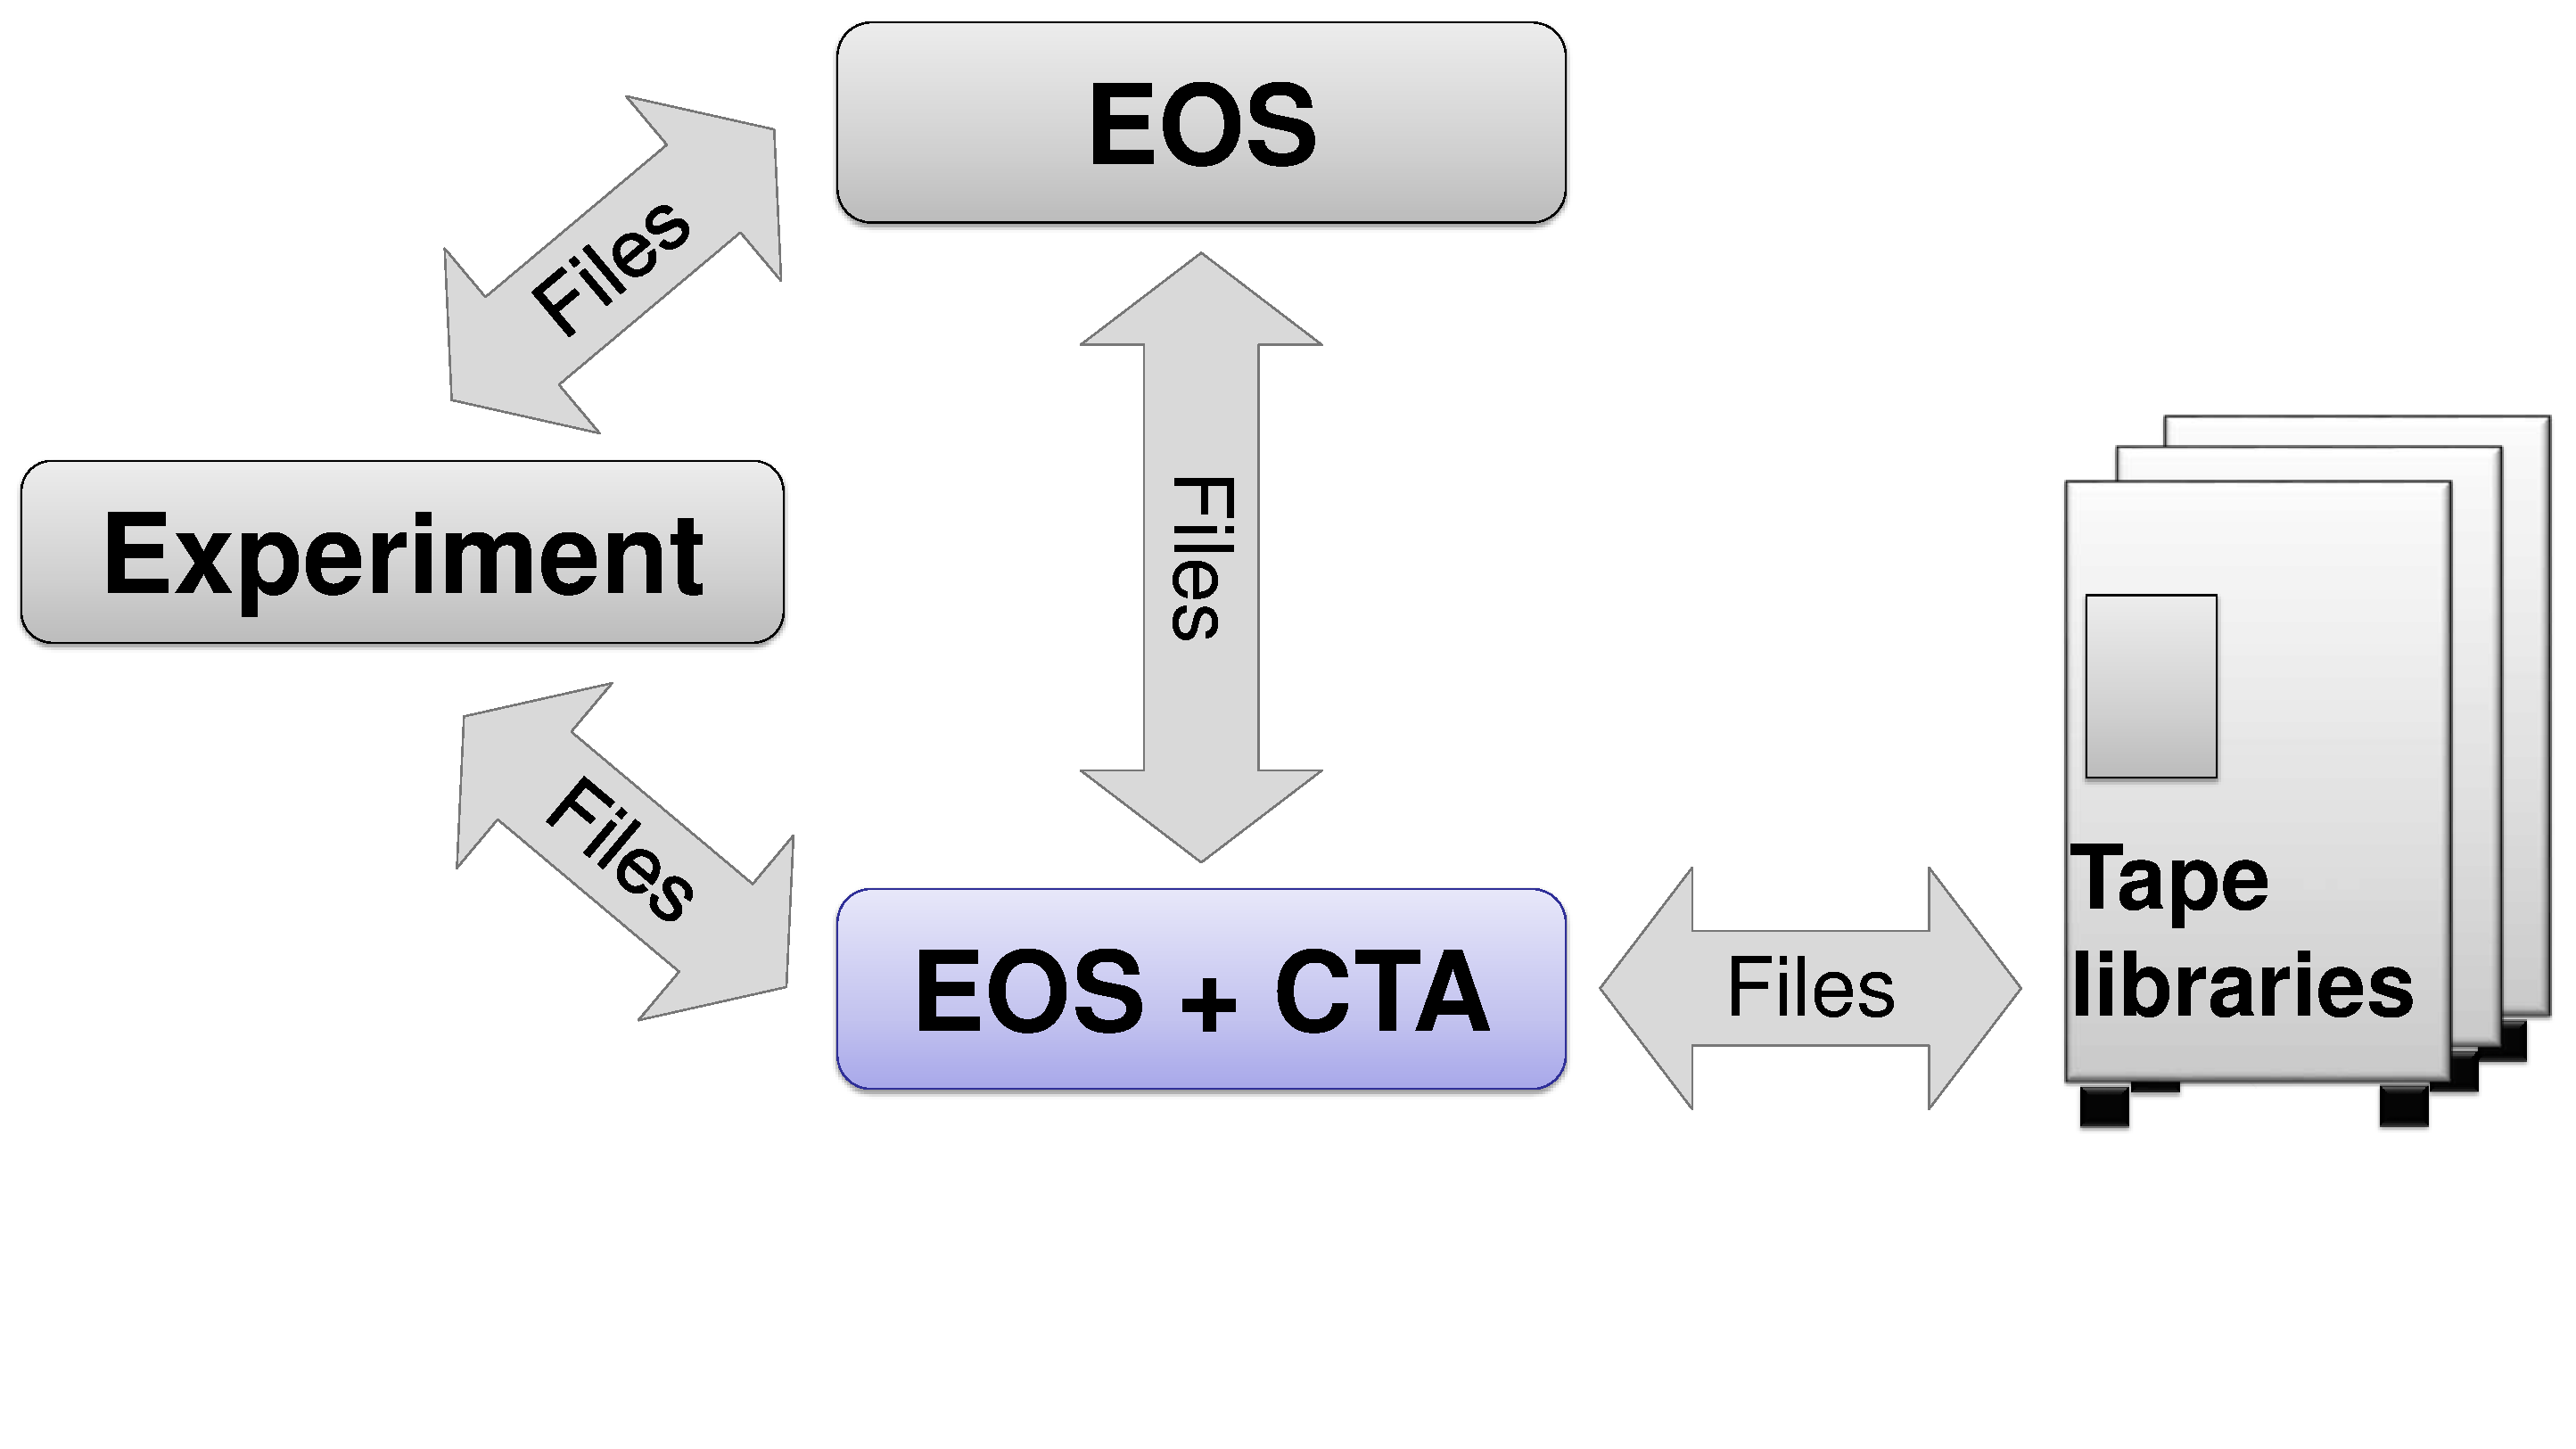
\includegraphics[scale=0.18, trim=0mm 60mm 0mm 0mm, clip]{CTA_drop_in_replacement_deployment.pdf}
\caption{\label{replacement}EOS and CTA as a drop in replacement for CASTOR}
\end{figure}

Once experiments have replaced their CASTOR instance with EOS and CTA they
will in fact have two EOS instances.  The original EOS instance for storing
files they work on and modify and the new EOS instance acting as a staging
area for the CTA tape backend. Figure \ref{consolidated} shows that instead and
at the choice of an experiment and the IT operations teams, the two EOS
instances could be merged into one.

\begin{figure}[h]
\centering
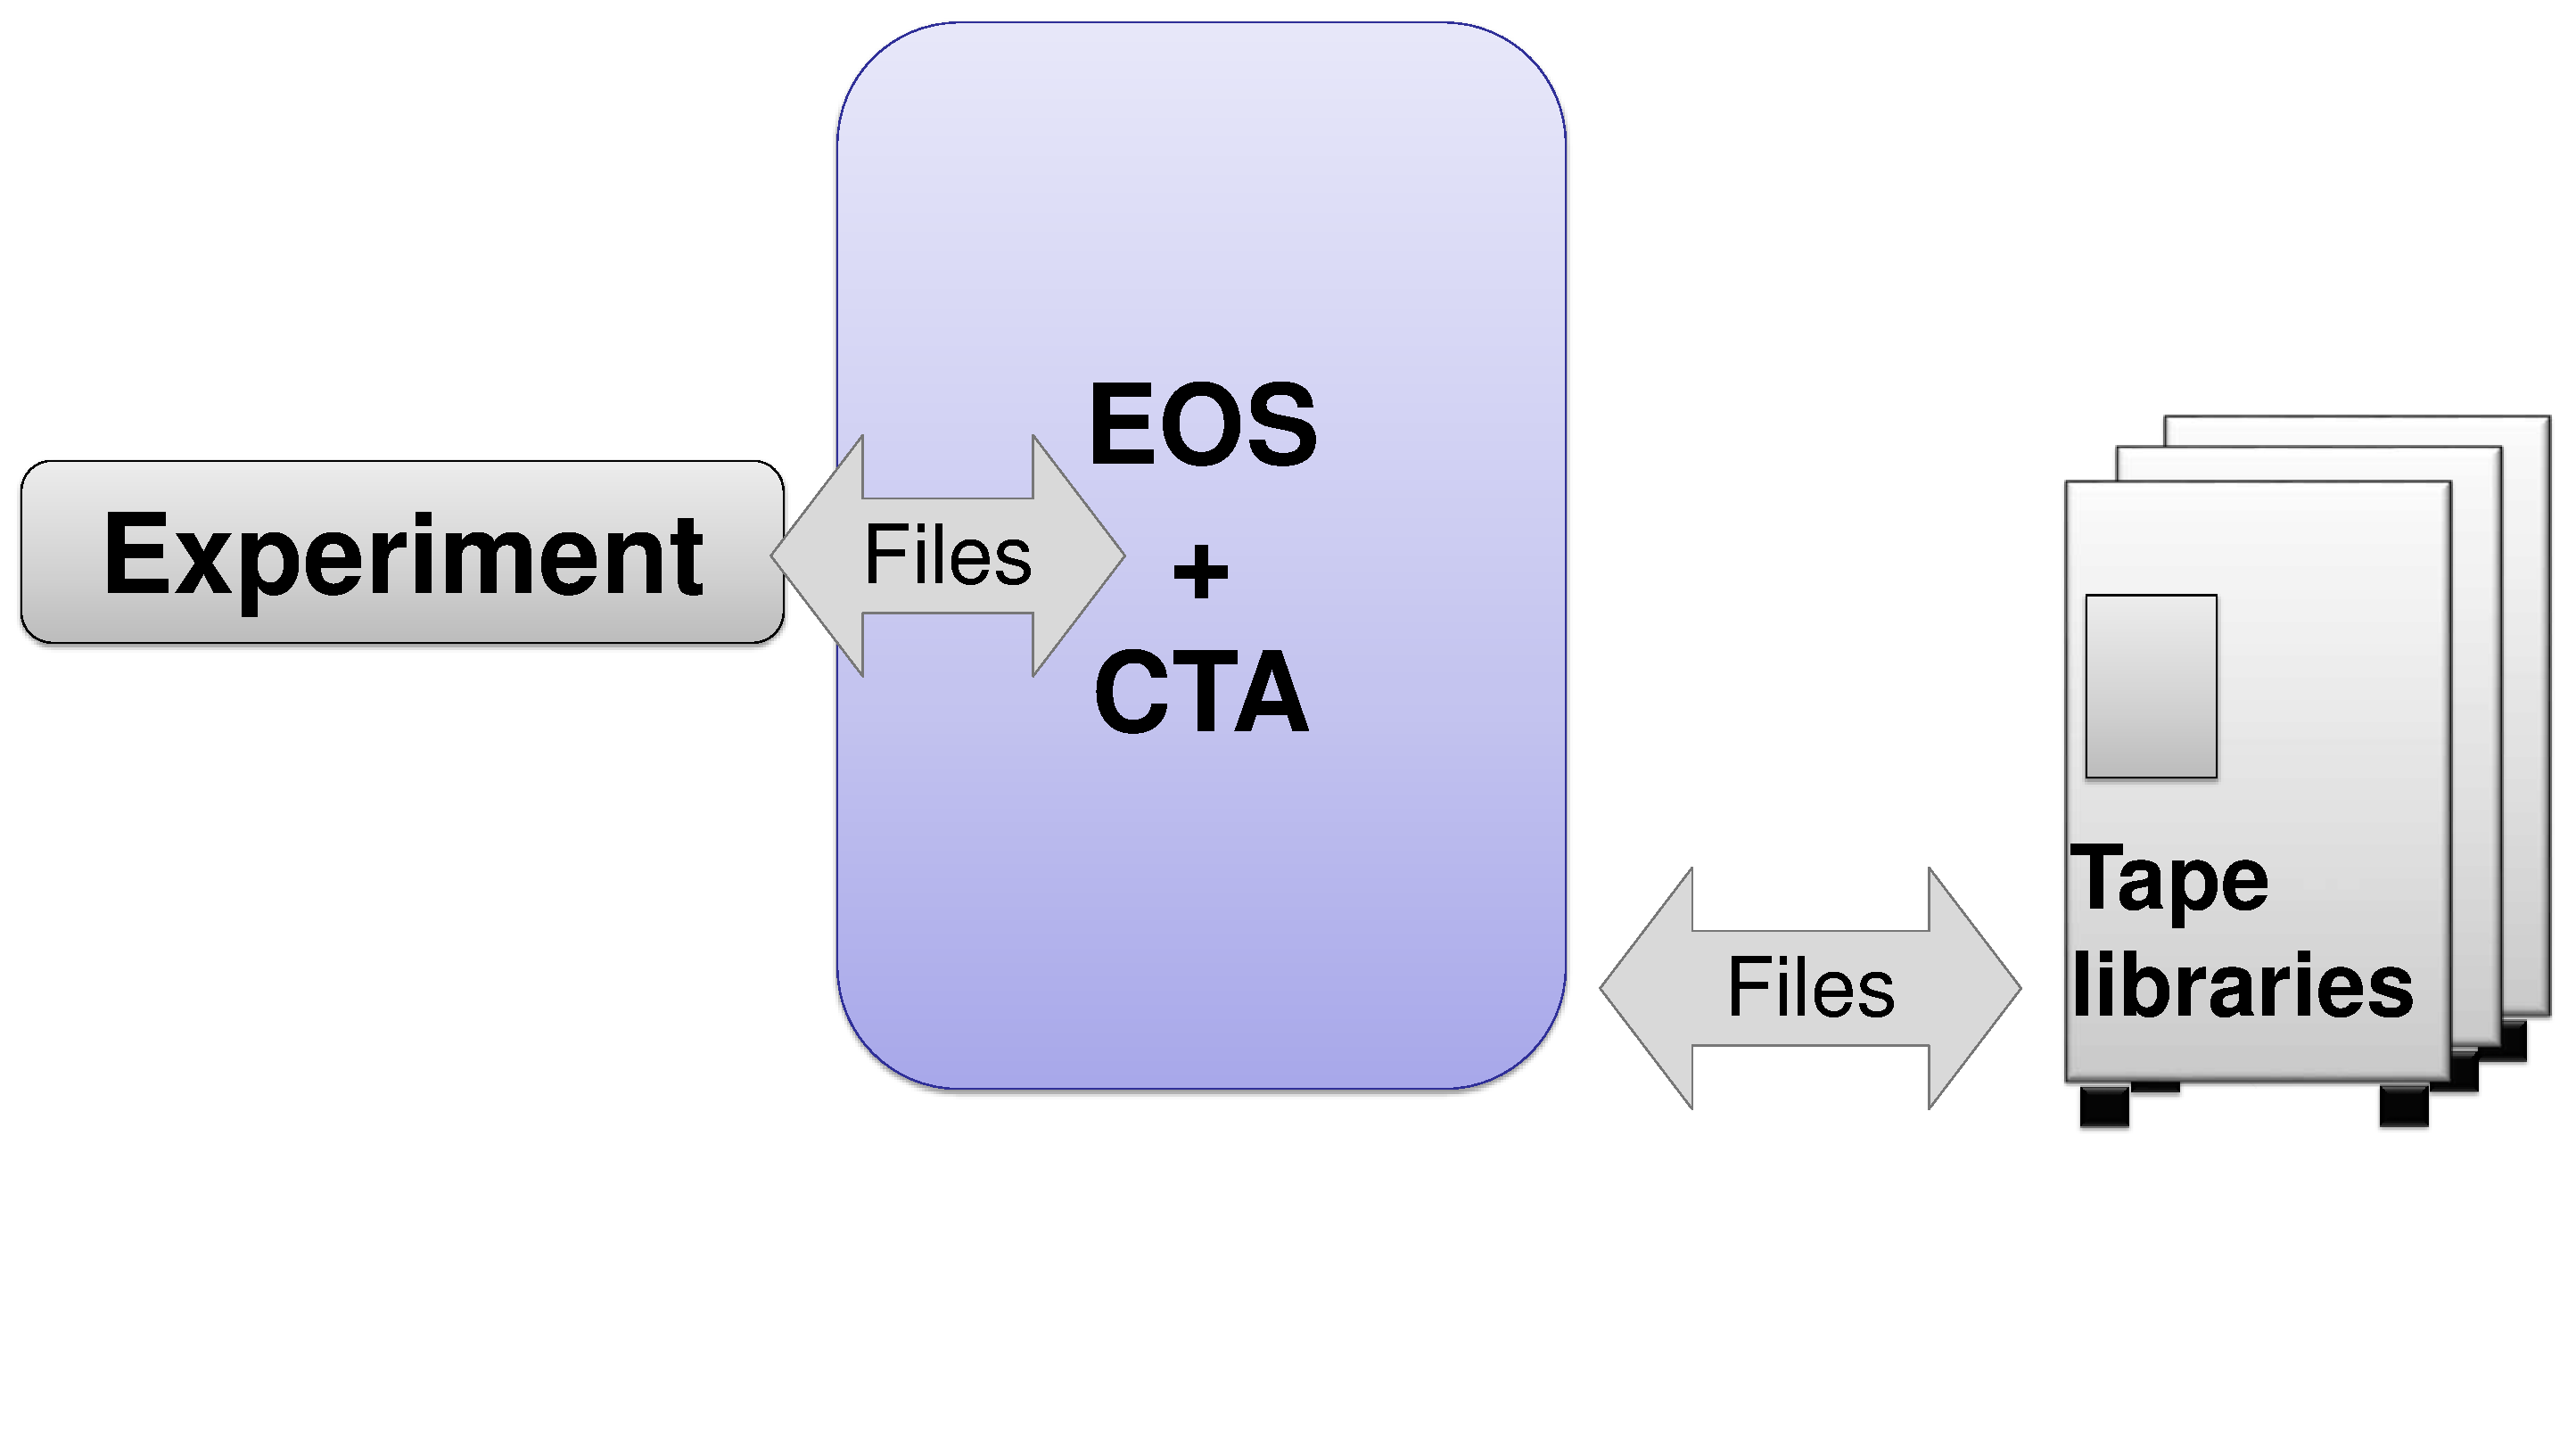
\includegraphics[scale=0.18, trim=0mm 60mm 0mm 0mm, clip]{CTA_consolidated_deployment.pdf}
\caption{\label{consolidated}Consolidate EOS if desired}
\end{figure}

CASTOR currently stores the custodial copy of all LHC physics data on tape.
CASTOR and CTA share the same tape format.  This means only the metadata
needs to be copied from CASTOR to EOS and CTA, no files needs to be copied
between CASTOR and CTA tapes.  CTA will simply take ownership of CASTOR
tapes as they are migrated from CASTOR to CTA.

The milestones for the CTA project are as follows.  In the second quarter of
2017 an internal release of CTA will be made that is intended for redundant use
cases within the IT-ST  group such as additional backups of filer data (AFS/NFS)
and additional copies of data from the Large Electron Position collider (LEP).
In the second quarter of 2018 the first production release of CTA will be made.
This release will have the ability to repack tape media and is intended to
migrate small virtual organizations such as non-LHC experiments from CASTOR to
EOS and CTA.  Finally in the fourth quarter of 2018, the second production
release of CTA will be made.  This release will be used to migrate large virtual
organizations such as LHC experiments from CASTOR to EOS and CTA.

\section{Conclusion} \label{conclusion}

CTA will avoid functional duplication with EOS through a clean, consolidated
separation between disk and tape.  EOS will focus on providing high-performance
disk storage, data transfer protocols and meta-data operations.  CTA will focus
on providing efficient tape backend storage.

CTA will introduce pre-emptive drive scheduling which will automatically
schedule the background tasks of tape media repacking and data verification.
This automatic scheduling will use the tape drives at full speed all of the time
and therefore enable CTA to cope with the 150 petabytes per year data rate of
LHC physics run 3.

CASTOR and CTA share the same tape format.  This means migrating data from
CASTOR to EOS and CTA only requires the metadata to be copied and CTA taking
ownership of CASTOR tapes.

In addition to the hierarchical namespace of EOS, CTA will have its own flat
catalogue of every file archived to tape.  This redundancy in metadata will
provide an additional recovery tool in the event of a disaster.

The architecture of CTA has benefited from a fresh start.  Without the need to
preserve the internal interfaces of the CASTOR networked components, CTA has
been able to reduce the number of networked components in the tape storage
system.

LHC experiments can expect to start migrating from CASTOR to EOS and CTA at the
beginning of 2019 which is the beginning of the long shut down period between
LHC physics runs 2 and 3.

\section{References}

\begin{thebibliography}{9}
\bibitem{CASTOR} CASTOR homepage {\it http://cern.ch/castor}
\bibitem{experiences} Cancio G, Bahyl V, Kruse D F, Leduc J, Cano E and Murray S 2015 Experiences and challenges running CERN's high capacity tape archive \textit{J. Phys.: Conf. Series}  \textbf{664} 042006
\bibitem{EOS} EOS homepage {\it http://cern.ch/eos}
\bibitem{new} Cano E, Murray S, Kruse D F, Kotlyar V and C\^{o}me D The new CERN tape software - getting ready for total performance \textit{J. Phys.: Conf. Series} \textbf{664} 042007 
\bibitem{repack} Kruse D F 2013 The repack challenge {\it Jour. of Phys.: Conf. Ser.} \textbf{513} 042028
\end{thebibliography}

\end{document}
